\begin{figure}[htbp]
\centering
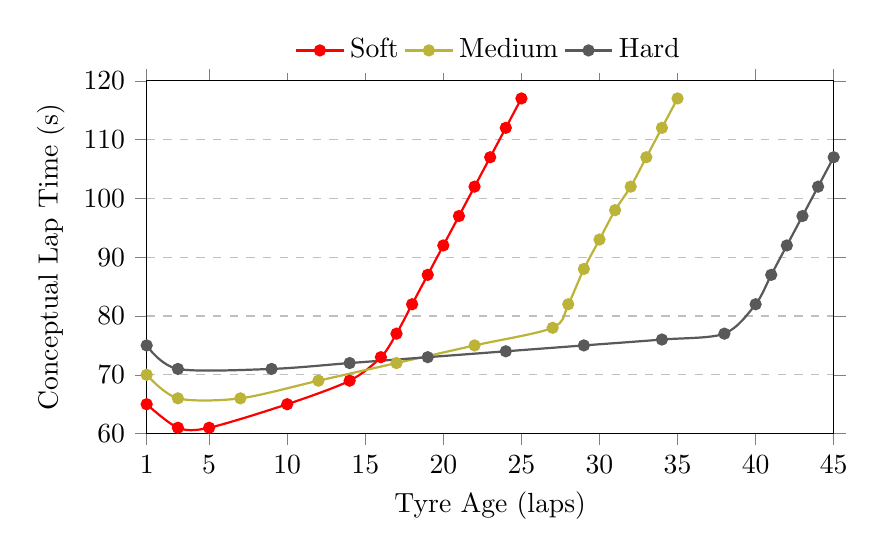
\begin{tikzpicture}
\begin{axis}[
    width=0.85\textwidth,
    height=0.5\textwidth,
    xlabel={Tyre Age (laps)},
    ylabel={Conceptual Lap Time (s)},
    xmin=1,
    xmax=45,
    ymin=60,
    ymax=120,
    ytick={60,70,80,90,100,110,120},
    xtick={1,5,10,15,20,25,30,35,40,45},
    ymajorgrids=true,
    grid style=dashed,
    legend style={
        at={(0.5,1.02)},
        anchor=south,
        legend columns=3,
        draw=none
    },
    tick align=outside
]

% Soft
\addplot[
    thick,
    red,
    smooth,
    mark=*,
    mark size=1.8pt
] coordinates {
(1,65)
(3,61)
(5,61)
(10,65)
(14,69)
(16,73)
(17,77)
(18,82)
(19,87)
(20,92)
(21,97)
(22,102)
(23,107)
(24,112)
(25,117)
};
\addlegendentry{Soft}

% Medium
\addplot[
    thick,
    yellow!70!black,
    smooth,
    mark=*,
    mark size=1.8pt
]  coordinates {
(1,70)
(3,66)
(7,66)
(12,69)
(17,72)
(22,75)
(27,78)
(28,82)
(29,88)
(30,93)
(31,98)
(32,102)
(33,107)
(34,112)
(35,117)
};
\addlegendentry{Medium}

% Hard
\addplot[
    thick,
    black!65,
    smooth,
    mark=*,
    mark size=1.8pt
]  coordinates {
(1,75)
(3,71)
(9,71)
(14,72)
(19,73)
(24,74)
(29,75)
(34,76)
(38,77)
(40,82)
(41,87)
(42,92)
(43,97)
(44,102)
(45,107)
(46,112)
(47,117)
};
\addlegendentry{Hard}

\end{axis}
\end{tikzpicture}
\caption{Conceptual tyre degradation curves used by the strategy model. Soft tyres provide the greatest initial performance but degrade most rapidly, while hard tyres exhibit the lowest initial performance and slowest degradation.}
\label{fig:1_conceptual_tyres}
\end{figure}